\documentclass[12pt]{article}  
%%Read the manual for other options. 

\pagestyle{empty} %%Eliminates page numbers
%%\input rmb_macros
%%Collect your favorite macros in a 
%%separate file

%\input amssym.def
%\input amssym
%\input mssymb
%%Defines additional symbols



\usepackage{graphics}
\usepackage{amsmath,amssymb,amsthm, multicol,tikz,pgf,subfig,enumerate}
\usetikzlibrary{arrows.meta}
%\usepackage[pdftex]{graphicx}
\usepackage{epsf}
\newenvironment{theorem}
{\begin{proof}[Theorem]}
{\end{proof}}
%%Use to include pictures. 

%\newcommand{\comment}[1]{}
%\newcommand{\sobolev}[2]{W^{#1,#2}}
%\newcommand{\sobolev}[2]{L^#2_#1}
%%Some examples of macros or new commands.

%\addtolength{\oddsidemargin}{-.75in}
%\addtolength{\evensidemargin}{-.75in}
%\addtolength{\textwidth}{1.5in}
%\addtolength{\topmargin}{-1in}
%\addtolength{\textheight}{2.25in}
%%Set margins, defaults are ok. 

\begin{document}
\begin{center}
{\bf \Large Public-Key Cryptography}
\vspace{0.2cm}
\hrule
\end{center}

\section*{Suppose...}
...that your friend's birthday is coming up. They've gone off to college on the other side of the country, and so that you don't start to drift apart, you want to send them a cake. They're living in a not-so-great part of town and you want to make sure nobody who isn't your friend opens the vulnerable package on their doorstep.\\

\noindent You have some padlocks and their corresponding keys. Why not try locking the box and sending it off to them then? Then no unwanted party can get to the cake. Well unfortunately neither can the wanted party -- your friend. However, your friend has padlocks of their own.

\subsection*{Question 1}
What can you and your friend do to ensure that your friend \textit{and only your friend} can open the box with the cake in it?

\vspace{3cm}

\section*{Graphs}
A \textbf{graph} is made of \textbf{vertices} (the plural of \textbf{vertex}) and \textbf{edges} between them. We can think of a vertex as just being a single point. An edge joining vertex $v_1$ to $v_2$ is represented by the pair $(v_1, v_2)$. Here we say that $v_1$ is \textbf{adjacent} to $v_2$ or that $v_1$ and $v_2$ are \textbf{neighbors}. We can visualize a graph by representing its vertices by points and its edges as line segments or curves connecting these points.\\

\noindent Now say we have a set of five vertices, $V = \{v_1, v_2, \ldots, v_5\}$. We can form several graphs with these vertices, a couple of which are shown in Figure 1. Graph $(V, E_1)$ has the edges $E_1 = \{(v_1, v_2), (v_1, v_4), (v_3, v_4), (v_4, v_5)\}$.
\begin{figure}
    \centering
    \subfloat[$(V, E_1)$]{{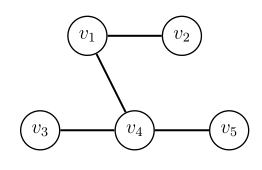
\includegraphics[scale=.7]{graph1} }}%
    \qquad
    \subfloat[$(V, E_2)$]{{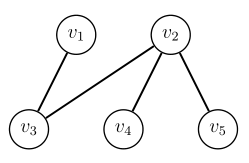
\includegraphics[scale=.7]{graph2} }}%
    \caption{Two graphs with the same set of vertices}%
    %\label{fig:example}%
\end{figure}


\subsection*{Question 2}
\begin{enumerate}[a]
	\item Write the edge set for the graph $(V, E_2)$.
	\vspace{1cm}
	\item For each vertex in the above graphs, list its neighbors.
	\vspace{1cm}
	\item If we insist that no vertex can be adjacent to itself and any two distinct vertices can be joined by at most one edge, how many possible graphs can we make with five vertices? What about with $n$ vertices?
	\vspace{1cm}
\end{enumerate}

\section*{The Plan\footnote{Teaching Fundamentals Concepts of Informatics: 4th International Conference on Informatics in Secondary Schools - Evolution and Perspectives, ISSEP 2010, Zurich, Switzerland, January 13-15, 2010. Proceedings (pp.112-123)}}
The plan is to use a graph to encode a message in a way that only the intended recipient can easily decode it. Here our messages are going to be numbers (this isn't really that much of a limitation. Why not?).\\

\noindent Suppose we want to disguise the number 113 with the graph given in Figure 2a. We start by splitting the number 113 into ten pieces -- one per vertex. These pieces can be whatever we want them to be as long as they sum to 113. We assign each piece to a vertex as in Figure 2b. Clearly our original number, 113, is easily reconstructed from these pieces. Just add them up.

\begin{figure}
    \centering
    \subfloat[Starting Graph]{{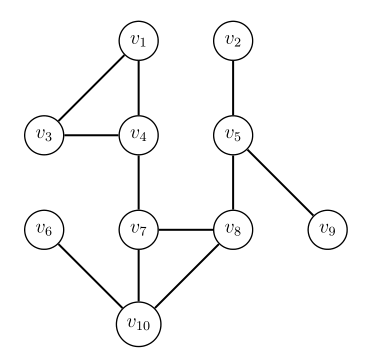
\includegraphics[scale=.6]{pk1} }}%
    \qquad
    \subfloat[Message]{{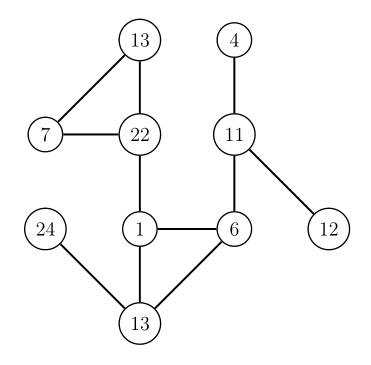
\includegraphics[scale=.6]{m1} }}%
    \\
    \subfloat[Ciphertext]{{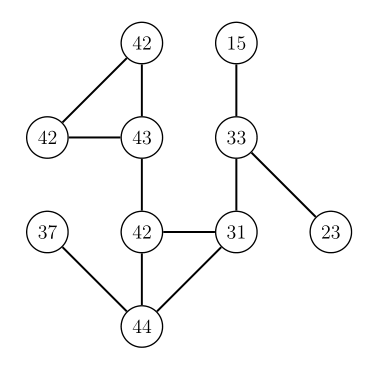
\includegraphics[scale=.6]{c1}}}
    \caption{Using a graph to encrypt a message.}%
    %\label{fig:example}%
\end{figure}
\noindent Now let's scramble our message. To do this, we add to each vertex the sum of its neighbors. So for example, if a vertex contains the number 6 and its three neighbors have numbers 11, 5, and 17, then we replace the 6 with $6+11+5+17 = 39$. This process of scrambling our message is called \textbf{encryption} and the resulting numbered graph is called the \textbf{ciphertext}.\\

\noindent While we could just add up all the numbers in our original graph to reconstruct our message, there doesn't seem to be an obvious way to get 113 from the ciphertext. But maybe you can figure one out.\\

\section*{Cryptanalysis}

\noindent Let's try some \textbf{cryptanalysis}: decrypting a ciphertext without knowing any decryption algorithm in advance. You and a partner will be given two copies of the same graph. Choose a number and repeat the process we walked through above. Assign a number to each vertex so that all vertices sum to your chosen number. Then walk through the encryption process and record the ciphertext on the second graph.\\

\noindent Once every team has encrypted their secret number, we'll exchange ciphertexts. Try to see if you can recover the original message from the ciphertext you're handed.

\newpage

\section*{Decryption and Exact Dominating Sets}
The graphs you were handed were carefully designed so that the encryption process can be quickly reversed if some secret information is known. Returning to the message and ciphertext in Figure 2, we see that the numbers in vertices $v_4$, $v_5$, and $v_6$ sum to the secret number 113: $37 + 43 + 33 = 113$.\\

\noindent The vertices $v_4$, $v_5$, and $v_6$ form what we'll call an  \textbf{exact dominating set}. An exact dominating set, $D$, of a graph $(V, E)$ is a subset of vertices so that each vertex in $V$ that isn't in $D$ is adjacent to \textit{exactly one} vertex in $D$ and no two vertices in $D$ are adjacent to one another.
% \begin{figure}[h]
% 	\centering
% 	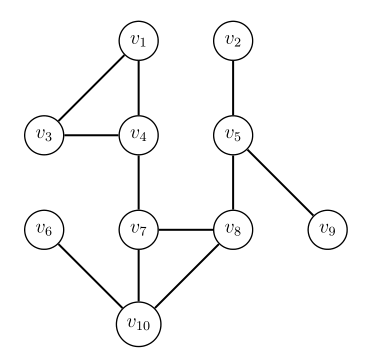
\includegraphics[scale=.5]{pk1}
% 	\caption{}
% \end{figure}

\subsection*{Question 3}
\begin{enumerate}[(a)]
	

	%\newpage
	
	\item Determine if each graph has an exact dominating set.
	\begin{figure}[h]
    \centering
    \subfloat[]{{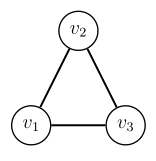
\includegraphics[scale=.6]{3a1} }}%
    \qquad
    \subfloat[]{{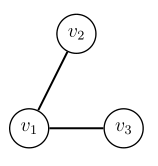
\includegraphics[scale=.6]{3a2} }}%
    \\
    \subfloat[]{{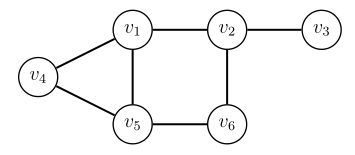
\includegraphics[scale=.6]{3a3}}}
    \qquad
    \subfloat[]{{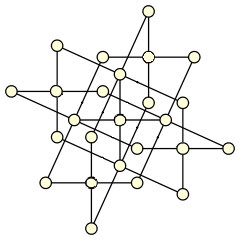
\includegraphics[scale=.7]{3a4}}}
    %\caption{Using a graph to encrypt a message.}%
    %\label{fig:example}%
	\end{figure}

	\item Draw a graph with five vertices that has an exact dominating set. What are the possible sizes for an exact dominating set in a graph with five vertices?
	%\vspace{3cm}

	\item Given integers $m$ and $n$, can you come up with a way to draw a graph with $m+n$ vertices that has an exact dominating set of size $m$?

	\vspace{3cm}

	\item Suppose you're given a ciphertext made with a graph that has an exact dominating set. Explain \textit{why} summing the values on the exact dominating set reveals the message.

	\vspace{3cm}

	\item A \textbf{dominating set}, $D'$, of a graph is a subset of its vertices such that each vertex not in $D'$ is adjacent to at least one vertex in $D'$. Explain how this is different from an \textit{exact} dominating set, maybe by drawing a graph that has a dominating set that isn't an exact dominating set. Why is it important that we use exact dominating sets for our encryption scheme?

	\vspace{3cm}
\end{enumerate}

\section*{Putting it Together}
Public-key cryptography is the process of encrypting and decrypting messages in such a way that \textit{anybody} can encrypt a given message but only the recipient can decrypt it. To accomplish this, the recipient, Alice, publishes her \textit{public key} for the world to see -- it isn't kept secret. If Bob has Alice's public key, he can use it to encrypt a message and send it to Alice, who decrypts it using her secret \textit{private key}.\\

\noindent The advantage to this system is that no sensitive information is ever transfered unmasked. Alice doesn't care if an eavesdropper, Eve, sees her public key. If the underlying encryption algorithm is any good, if Eve intercepts Bob's encrypted message to Alice, she won't be able to decipher it if she doesn't have Alice's private key.

\subsection*{Question 4}
\begin{enumerate}[(a)]
	\item Consider the graph-based encryption scheme we discussed earlier. How is this a public-key system? What part constitutes the public key and what part is the private key? Is it hard to find the private key if you know only the public key? How can Alice and Bob use this system to communicate in the presence of an eavesdropper, Eve?

	\vspace {3cm}

	\item Suppose Alice and Bob have access to many different colors of paint. Alice and Bob \textit{publicly} agree on the color yellow. Alice \textit{secretly} chooses the color red and Bob \textit{secretly} chooses the color green. How can Alice and Bob publicly communicate and use the paints they've chosen to establish a shared secret color, even if Eve listens in on their conversation?
\end{enumerate}

\newpage

\section*{Bonus Material: Number Theory}
Let $a$, $b$, and $n$ be positive integers. We say that $a$ is \textbf{congruent to} $b$ \textbf{mod} $n$ if $a$ and $b$ have the same remainder when divided by $n$. We write this as $a\equiv b\pmod{n}$. Here's a theorem about prime numbers.
\begin{theorem}
	Let $p$ be a prime number and let $a$ be an integer not divisible by $p$. Then there exists a number $b$ such that $ab\equiv 1\pmod{p}$.
\end{theorem}

\noindent Here's another theorem often attributed to the French mathematician Fermat:
\begin{theorem}(Fermat's little theorem)
	Let $p$ be a prime number and let $a$ be an integer not divisible by $p$. Then $a^{p-1}\equiv a \pmod{p}$.
\end{theorem}



\section*{Question 5}
\begin{enumerate}[(a)]
	
	\item (A bit hard) Prove the first theorem. Hint: think about greatest common divisors and the Euclidean algorithm.
	\vspace{4cm}

	\item (Harder) Prove Fermat's little theorem. Hint: consider the sets \\$S = \{1, 2, \ldots, p-1\}$ and $aS = \{a, a\cdot 2, \ldots, a\cdot (p-1)\}$.
	

	\vspace{4cm}

	\item Suppose Bob wants to send a number $m$ to Alice. Use the two theorems above to construct a public-key system where Bob can securely send $m$ to Alice.\\

	\noindent Here's a good start. Alice and Bob publicly agree on a prime number $p$. Alice and Bob then secretly choose two numbers each. What properties should these numbers satisfy? How can Bob use his numbers to encrypt his message and how can Alice use her to decipher it?
\end{enumerate}






% \newpage
% \begin{tikzpicture}
% \begin{scope}[every node/.style={circle,thick,draw}]
%     \node (v1) at (2,2) {$v_1$};
%     \node (v2) at (4,2) {$v_2$};
%     \node (v3) at (6,2) {$v_3$};
%     \node (v4) at (0,1) {$v_4$};
%     \node (v5) at (2,0) {$v_5$};
%     \node (v6) at (4,0) {$v_6$};
% \end{scope}

% \begin{scope}[every node/.style={fill=white,circle},
%               every edge/.style={draw=black,very thick}]
%     \path (v1) edge (v2);
%     \path (v2) edge (v3);
%     \path (v4) edge (v1);
%     \path (v4) edge (v5);
%     \path (v5) edge (v1);
%     \path (v5) edge (v6);
%     \path (v6) edge (v2);
% \end{scope}
% \end{tikzpicture}


\end{document}